\scanpage{129}
ment define straight away
\[
\tag{206}
\begin{gathered}
\left\{\begin{aligned}
\mathcal D_*^*&=\coprod_{d_0\geq d_1\mathord{\cdot\,-\,-}\geq d_r\geq0}D^*_{d_0,d_1,-,d_r}\\
&=\text{inverse image of }D_*^*=\coprod_{d\in\mathbb N}D_d^*\text{ under}\\
&\quad\text{the morphism }\unsure{0|o}:\mathcal D_*\mathrel{\tikz[baseline=-.5ex,x=1em,y=1em]{\draw[line width=.4pt] (0,0)--(.9,0)--(.9,.13);}} D_*\\
&\quad\text{defined by the }D_{d_0,\mathord{\cdot\,-\,\cdot},d_r}\longrightarrow D_{d_0}
\end{aligned}\right.\\
\text{i.e. defined by the }\overset{\inserted{\text{``first vertex'' morphisms}}}{
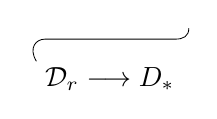
\begin{tikzpicture}[baseline=(m.base)]
\node[inner sep=0pt] (m) {$\mathcal D_r\longrightarrow D_*$};
\draw[line width=.3pt] ([xshift=-3pt,yshift=2pt]m.north west)
.. controls ([xshift=-6pt,yshift=7pt]m.north west) and ([xshift=-3pt,yshift=10pt]m.north west) .. ([yshift=10pt]m.north west)
-- ([yshift=10pt]m.north east)
.. controls ([xshift=3pt,yshift=10pt]m.north east) and ([xshift=5pt,yshift=11pt]m.north east) .. ([xshift=5pt,yshift=14pt]m.north east);
\end{tikzpicture}}
\end{gathered}
\]
\diagram{\begin{tikzcd}[ampersand replacement=\&,column sep=small,row sep=small]
\&\&\bullet\rlap{\(\,0\)}\arrow[d,no head]\\
\text{(transpose of}\&\underset{0}{\bullet}\arrow[ur]\&\bullet\rlap{\(\,1\)}
\arrow[d,no head,to path={(\tikztostart.south)--([yshift=2pt]\tikztotarget.center)--++(-.045,.04)\tikztonodes}]\&\text{)}\\
\&\&{}\rlap{\(\,2\)}\\
\&\&\vdots\arrow[d]\\
\&\&{}\rlap{\(\,r\)}
\end{tikzcd}}

We shall define
\[
\tag{207}
\left\{\begin{aligned}
P_{d_0,d_1,-,d_r}&=\text{inverse image of the }\overset{\underbrace{G_d\text{-}\unsure{\text{torsor}|\text{bundle}|\text{bundles}}}}{P_{d_0}}\text{ over }D_{d_0}\\
&\qquad\text{under }D_{d_0,\mathord{-\, -},d_r}\mathrel{\tikz[baseline=-.5ex,x=1em,y=1em]{\draw[line width=.4pt] (0,0)--(.9,0)--(.9,-.10);}} D_{d_0}\\
P^*_{d_0,d_1,\mathord{-\, -},d_r}&=P_{d_0,-,d_r}\mid D^*_{d_0,-,d_r}
\end{aligned}\right.
\]
\unsure{these are}\inserted{\unsure{indeed|are}} torsors under the Groups, \unsure{analytic|analytic}
(tori)
\[
\tag{208}
\begin{aligned}
G_{d_0,-,d_r}&=\text{inverse image of }G_{d_0}\\
&\quad\text{over }\unsure{D_0|d_0}\text{, under }D_{d_0,-,d_r}\mathrel{\tikz[baseline=-.5ex,x=1em,y=1em]{\draw[line width=.4pt] (0,0)--(.9,0)--(.9,.13);}} D_{d_0}\\
G^*_{d_0,-,d_r}&=G_{d_0,-,d_r}\mid D^*_{d_0,-,d_r}\unsure{.|-}
\end{aligned}
\]
We thus have a $2$-cartesian diagram of groupoids
\diagram{\(\bigl(\unsure{209}\bigr)\quad\)
\begin{tikzcd}[ampersand replacement=\&,column sep=large,row sep=large]
\bigl(\widetilde\Pi_{d_0\unsure{-}d_r}\overset{\mathrm{definition}}{=}\unsure{\Pi_1|\pi_1}P^*_{d_0,\mathord{-\, -},d_r}
\arrow[r]\arrow[d]
\&\unsure{\Pi_1|\pi_1}P^*_{d_0}\bigl(\overset{\mathrm{definition}}{=}\widetilde\Pi_{d_0}\bigr)\arrow[d]\\
\Pi_{d_0,-d_r}=\unsure{\Pi_1|\pi_1}\unsure{D_{d_0,-,d_r}|D^*_{d_0,-,d_r}}
\arrow[r,no head,to path={(\tikztostart.east)--([xshift=-2pt]\tikztotarget.west)--++(0,.055)\tikztonodes}]
\&\unsure{\Pi|\pi}D_{d_0}\bigl(\overset{\unsure{\mathrm{definition}|\mathrm{definition}}}{=}\Pi_{d_0}\bigr)
\arrow[ul,phantom,"2\text{-cartesian}" description]
\end{tikzcd}}
\margin{128}
